\chapter{Introduction}
The focus of this dissertation is on hand tracking, and specifically the merits of using synthetic data for training hand tracking systems. A hand tracking system is one that can automatically estimate the 3D locations of the joints in the hand, given an image of that hand. The overall purpose of a hand tracking system is to enable human-computer interaction with a hand as a medium (other forms of human-computer interaction include the use of keyboards, mice, and punchcards). Figure \ref{fig:intro:htex} illustrates an example of hand tracking for interaction with a Virtual Reality headset.

Recent hand tracking systems have become more accurate and robust, however these systems suffer under many scenarios such as from the ego-centric perspective (where the camera perspective of the hand is captured from a head-mounted camera, or similar positions). Hand tracking is notoriously difficult because the hand has many degrees of freedom (the different ways in which fingers can position themselves), and it can self-occlude (where one part of the hand blocks the view of another part of the hand in an image). Hand tracking systems require a lot of data to be able to perform well in different scenarios, but acquiring that data is difficult. While the process of capturing hand data is trivial, the challenge lies in annotating that data. For the type of hand tracking system mentioned above, annotating the data required to train a hand tracking system involves recording the 3D positions of a set amount of keypoints (known points in the hand that the hand tracking system is trying to predict the location of in 3D space, such as a knuckle). Manually labelling the data at scale is impossible in practical terms, particularly when the hand self-occludes, and recent attempts at manual annotation only offer limited resolution and size, \cite{wang2018mask} for example only managed 11703 images with 2D annotation, and they did not annotate self-occluded joint. Recent projects such as BigHand2.2M\cite{yuan2017bighand2} and ICVL\cite{tang2016latent} that automatically annotate datasets have collected millions of annotated images of hands, but they rely on a small amount of subjects, and there is no way of evaluating the accuracy of that annotation. Since the annotation is theoretically perfect, synthetic data offers a way to address the issue of accuracy and scale. Past attempts at generating synthetic data however lack the realism that real data can provide\cite{mueller2017real, malik2018deephps}. As mentioned by \cite{armagan2020measuring}, even with such large datasets, current systems still struggle to interpolate between poses in large datasets. More recently, the MANO model has attempted to address the lack of realism in synthetic hand data \cite{romero2017embodied}. Building on the previous work in full body rendering for computer graphics, the authors of MANO learn a synthetic hand data generation model based on real-world subjects, including hands interacting with objects.

\begin{figure}
    \centering
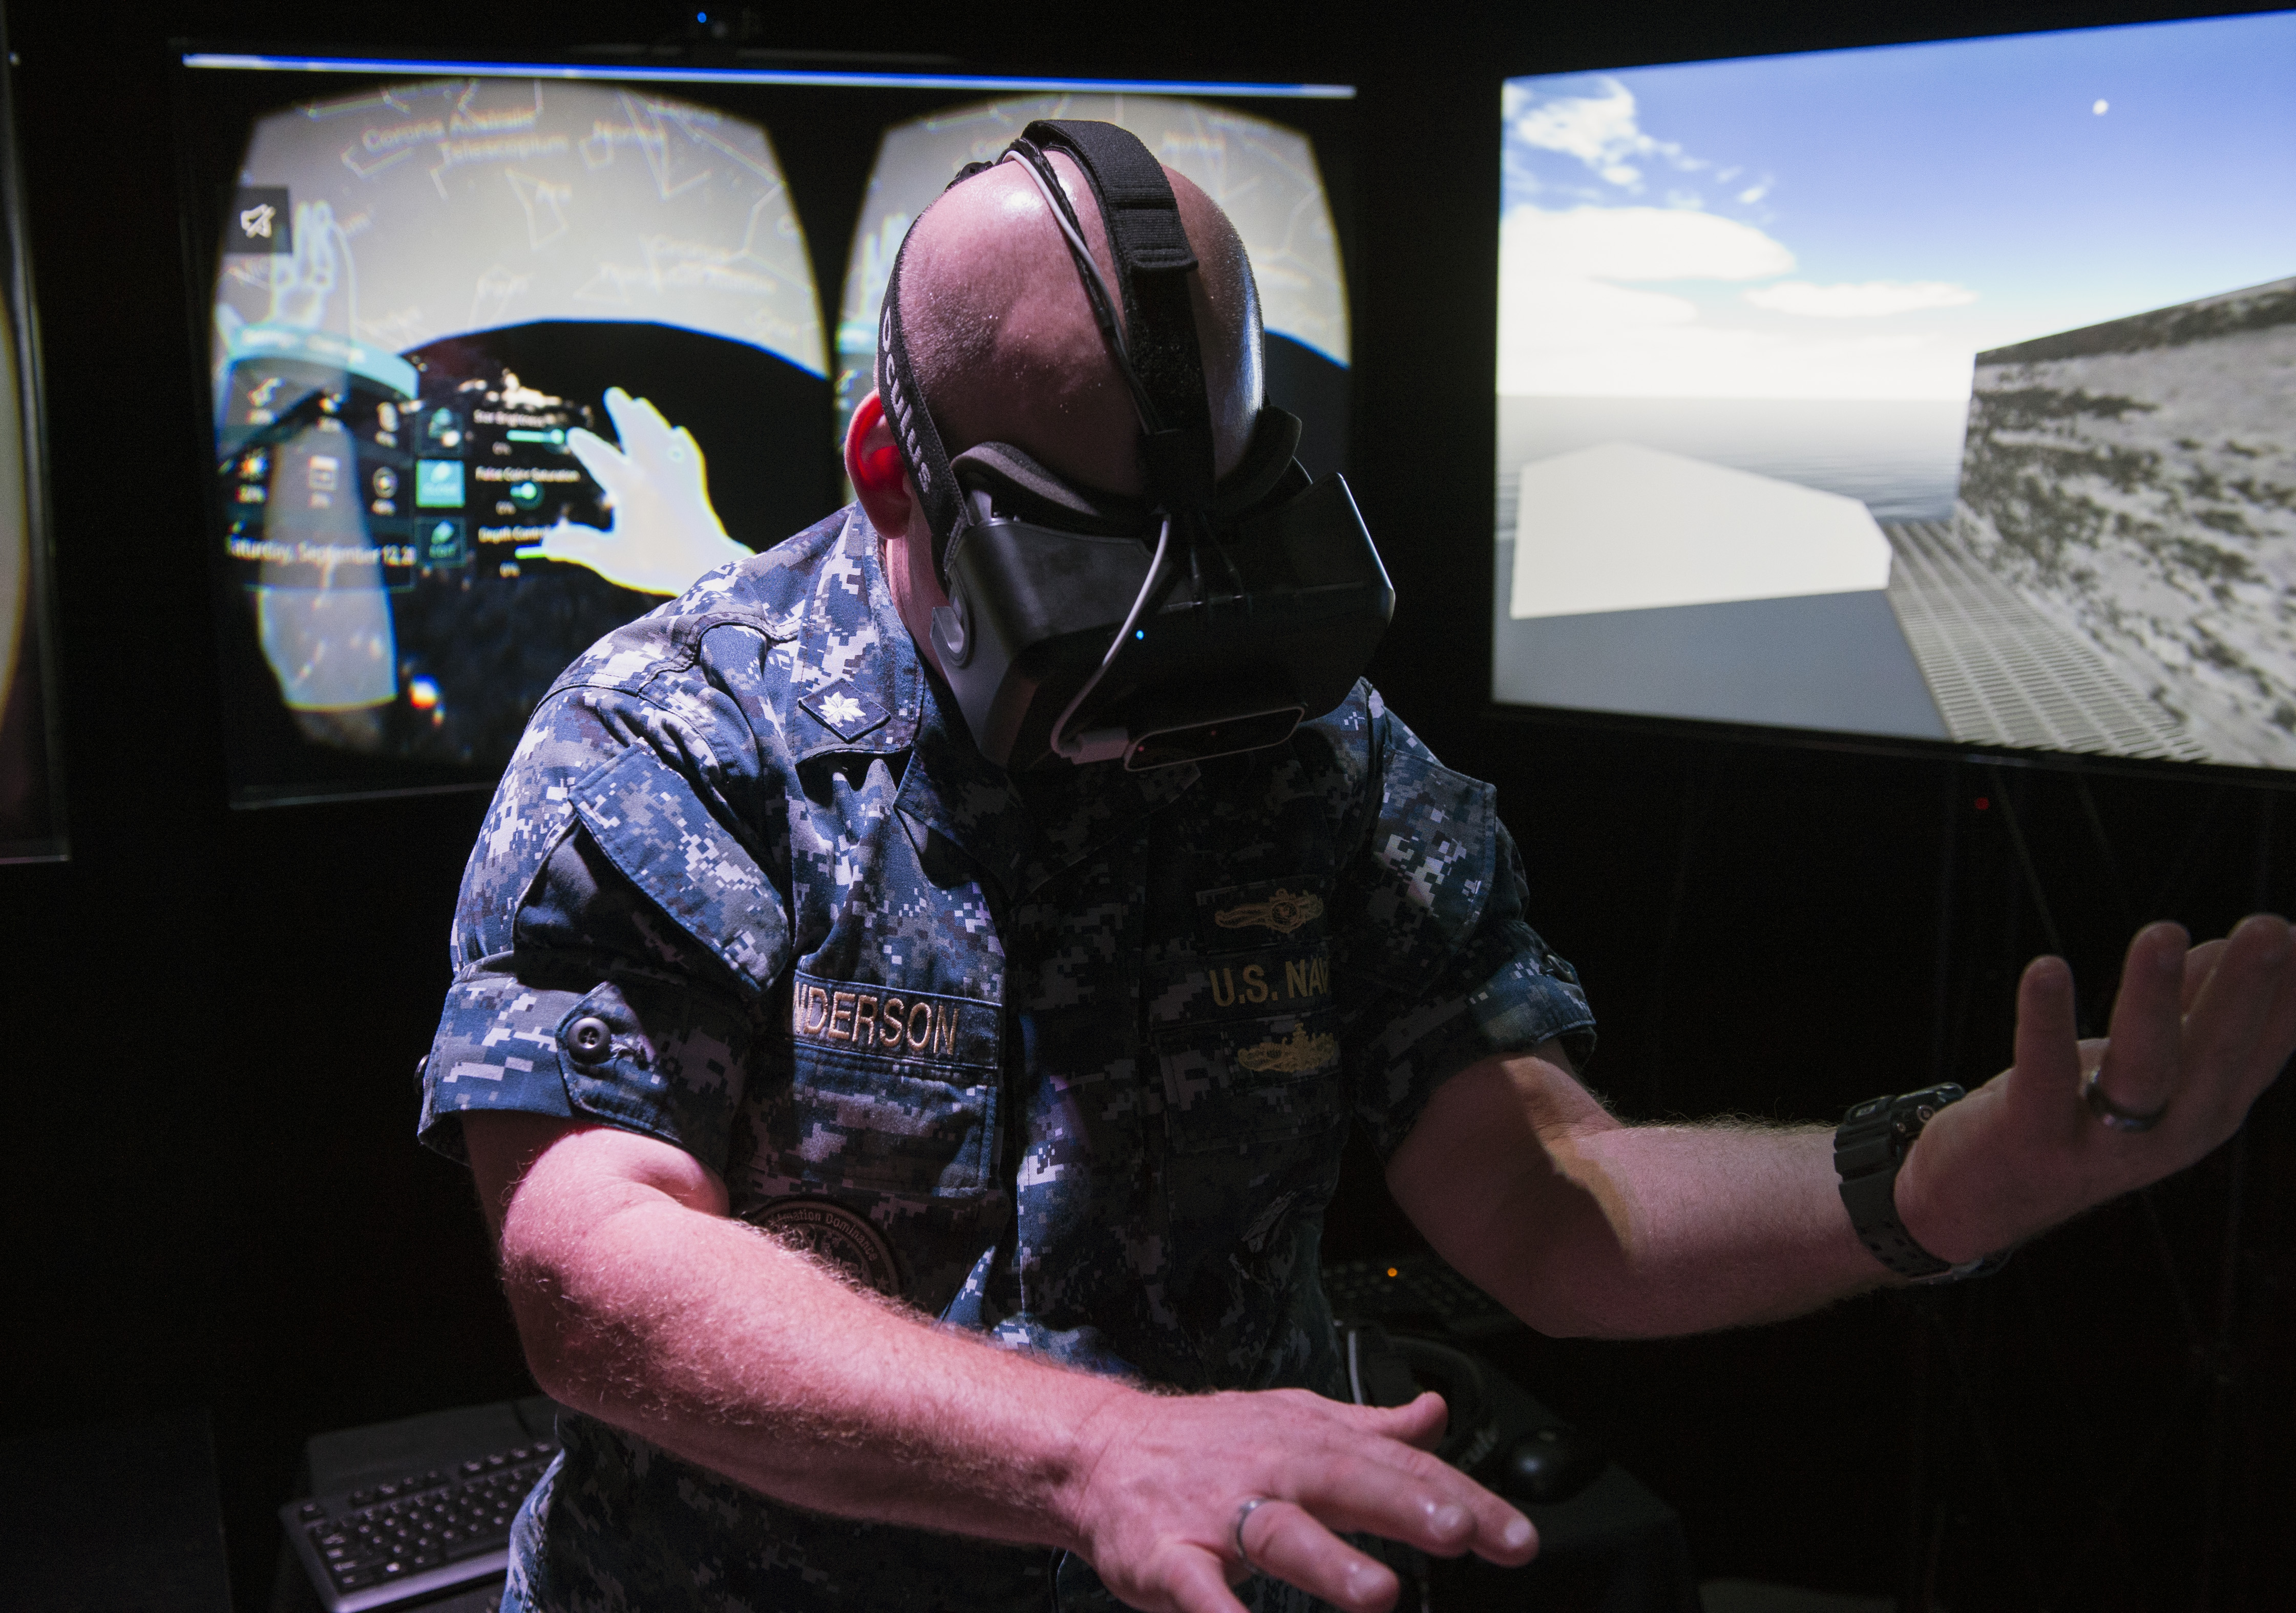
\includegraphics[width=400px]{figs/general/vr_example.jpg}
\caption{An example of the use of Virtual Reality using only hands to interface with the computer\protect\footnotemark.}
\label{fig:intro:htex}
\end{figure}
\footnotetext{CC-BY-2.0 License (\url{https://creativecommons.org/licenses/by/2.0/deed.en})\copyright$\,${\slshape John F. Williams} (title: 150914-N-PO203-142), obtained from \url{https://www.flickr.com/photos/usnavyresearch/23496662185/} (accessed 29th April 2020)}
% The goal of this dissertation is to investigate the current state of synthetic data generation methods for hand tracking systems using the MANO model. This is achieved by comparing the synthetic data with real data: the MSRA dataset\cite{sun2015cascaded}. The comparison is performed by training an existing hand tracking system, the V2V-Posenet model\cite{moon2018v2v}, with both kinds of data, and cross comparing the resultant models.

\section{Motivation}
\label{sec:intro:mot}
In recent years and decades, as computer technology has improved, new possibilities for human-computer interaction have emerged. This ranges from punch cards, to keyboards, to mice, and touch screens. The developments that these innovations have led to need not be enumerated here. Progress has been made in the development of new technologies and ways for human-computer interaction, which is being lead by the emergence of new technologies such as Augmented Reality (AR) and Virtual Reality (VR). While both technologies have been around for some time, one problem with them is how a user interacts with them. The use of human hands offers the potential to improve the human-computer interaction with these technologies, but hand tracking notoriously difficult problem. More recently, as of writing the world is under lockdown due to Covid-19. Computer mice and keyboards, due to the need to touch them are inevitable vectors of disease, and interacting with a computer using hand gestures alone offers a less risky way of using them. 

The specific motivation about using synthetic data to train a hand tracking system in this project is largely influenced by the {\slshape 5th International Workshop on Observing And Understanding Hands in Action} ({\slshape Hands 2019})\footnote{\url{https://sites.google.com/view/hands2019/home} (accessed 29th April 2020)}. The goals of this challenge are discussed more formally in \cite{armagan2020measuring}. The {\slshape Hands 2019} challenge provides three different tasks for: depth-based hand pose estimation, depth-based hand pose estimation with hands interacting with objects, and RGB-based hand pose estimation with hands interacting with objects. In all three of these tasks, participants are encouraged to use the MANO model to train with synthetic data.

\section{Objectives}
The objective of this dissertation is to evaluate the current state of generating synthetic data in 2020 towards improving the performance of hand tracking systems. This is achieved by comparing synthetic data generated with real data: the MSRA dataset \cite{sun2015cascaded}. The comparison is performed by training an existing hand tracking system, the V2V-Posenet model \cite{moon2018v2v}, with both kinds of data, and cross comparing the resultant models using a performance metric. The performance metric is Mean Squared Error (MSE), and is discussed in Section \ref{sec:pm}.



% While there have been previous attempts at generating synthetic datasets for hand tracking systems, this is to my knowledge the first time that a side-by-side comparison has been performed with a real hand tracking dataset to asses its quality.

\section{Overview}
Two synthetic data generation strategies are investigated. The first strategy generates the data based on random parameters for MANO, this is referred to as the {\slshape Random MANO Dataset}. The second strategy generates the data based on parameters determined from the groundtruth of the real dataset to recreate that real dataset using inverse kinematics, this is referred to as the {\slshape IK MANO Dataset}.

The key contributions of this dissertation are 
\begin{enumerate}
    \item Generating a new synthetic dataset using the MANO model.
    \item Performing a side-by-side comparison between a synthetic and real hand tracking dataset using the state-of-the-art synthetic hand data generation method, MANO.
    \item Providing a new framework for generating a synthetic dataset by using a real dataset as a basis.
\end{enumerate}

The rest of this dissertation is divided as follows. Section \ref{chap:lit} discusses and evaluates the previous work around hand tracking systems and datasets. Section \ref{chap:sd} discusses the underlying theory of what synthetic data is, the implications of training a hand tracking system with it, and the strategies used to generate such data. Section \ref{chap:es} discusses the practical details of the experimental setup used for this dissertation. Section \ref{chap:res} presents the results of the experiments to compare the synthetic and real dataset. Section \ref{chap:con} concludes this dissertation.


% Hand tracking systems have become ever more sophisticated \cite{}, however a 

% The key contributions of this dissertation are (1) framing an alternative approach to training a hand tracking system through transfer learning, (2) performing a side-by-side comparison between a synthetic and real hand tracking dataset, and (3) providing a new framework for generating a synthetic dataset by using a real dataset as a basis.

% \section{Hand Tracking}
% What is hand tracking, what are its goals, compare rgb and depth, describe the hollistic pipeline.
% Any background

% \section{Goals}
% Why am I making synthetic data, what are the goals